\question{Полупроводниковые лазеры и лазеры на свободных электронах.}

\subquestion{Полупроводниковые лазеры}

\emph{Полупроводниковый лазер} -- это лазеры с усиливающей средой на основе 
полупроводников, где генерация происходит, как правило, за счет вынужденного 
излучения фотонов при межзонных переходах электронов в условиях высокой 
концентрации носителей в зоне проводимости. 

В полупроводниковом лазере накачка осуществляется:
\begin{itemize}
	\item непосредственно электрическим током (прямая накачка);
    \item электронным пучком;
    \item электромагнитным излучением.
\end{itemize}

\begin{figure}[h!]
    \center
    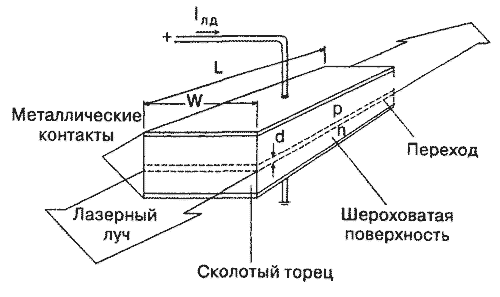
\includegraphics[width=.4\textwidth]{30_01}
\end{figure}

Без накачки большинство электронов находится в валентной зоне. Пучок накачки с 
фотонами с энергией немного больше ширины запрещенной зоны возбуждает 
электроны и переводит их в более высокоэнергетическое состояние в зоне 
проводимости, откуда они быстро релаксируют в состояние вблизи дна зоны 
проводимости. В то же время, дырки, генерируемые в валентной зоне, 
перемещаются в ее верхнюю часть. Электроны из зоны проводимости 
рекомбинируют с этими дырками, испуская фотоны с энергией, приблизительно 
равной ширине запрещенной зоны. Этот процесс может также стимулироваться 
входящими фотонами с подходящей энергией. Количественное описание основывается 
на распределении Ферми-Дирака для электронов в обеих зонах.

\subquestion{Лазеры на свободных электронах}

\emph{Лазер на свободных электронах (Free Electron Laser, FEL)} -- вид лазера, 
излучение в котором генерируется моноэнергетическим пучком электронов, 
распространяющимся в ондуляторе -- периодической системе отклоняющих 
(электрических или магнитных) полей. Электроны, совершая периодические 
колебания, излучают фотоны, энергия которых зависит от энергии электронов и 
параметров ондулятора.

\begin{figure}[h!]
    \center
    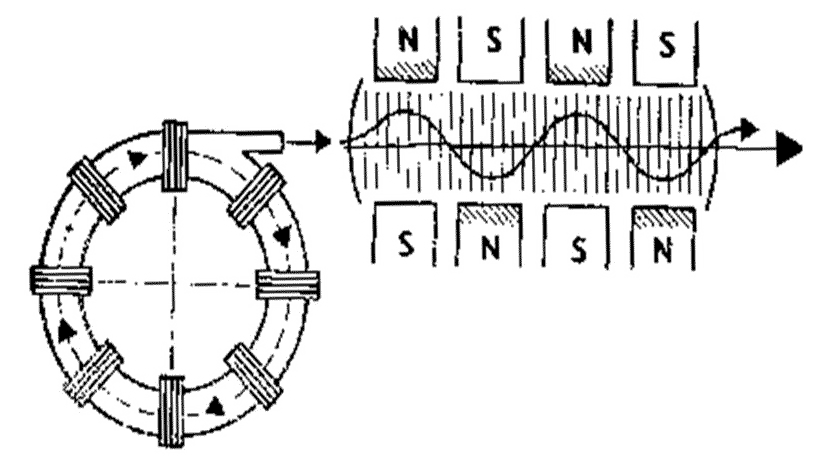
\includegraphics[width=.4\textwidth]{30_02}
\end{figure}

В отличие от газовых, жидкостных или твердотельных лазеров, где электроны 
возбуждаются в связанных атомных или молекулярных состояниях -- у FEL 
источником излучения является пучок электронов в вакууме, проходящий сквозь 
ряд расположенных специальным образом магнитов -- ондулятор, заставляющий 
пучок двигаться по синусоидальной траектории, теряя энергию, которая 
преобразуется в поток фотонов. В результате вырабатывается мягкое 
рентгеновское излучение, применяемое, например, для исследования кристаллов и 
других наноструктур.

Меняя энергию электронного пучка, а также параметры ондулятора (силу 
магнитного поля и расстояние между магнитами), можно в широких пределах менять 
частоту лазерного излучения, вырабатываемого FEL, что является главным 
отличием FEL от лазеров других систем. Излучение получаемое с помощью FEL 
применяется для изучения нанометровых структур -- есть опыт получения 
изображений частиц размером всего 100 нанометров. 

Для создания лазерного рентгеновского излучения необходим пучок электронов, 
разогнанный в синхротроне до скорости, близкой к скорости света. Полученный 
пучок направляется в специализированный прибор для генерации лазерного 
рентгеновского излучения -- вигглер.

Вигглер представляет собой магнит, создающий сильное поперечное (как правило, 
вертикальное) знакопеременное магнитное поле. Его можно представить себе как 
последовательность коротких дипольных магнитов, полярность каждого следующего 
из которых противоположна предыдущему. Вигглер устанавливается в прямолинейный 
промежуток электронного синхротрона, и ультрарелятивистский пучок проходит в 
нём по извилистой траектории, близкой к синусоиде, излучая фотоны в узкий 
конус вдоль оси пучка. Типичный диапазон длин волн синхротронного излучения, 
генерируемого вигглером, -- от жёсткого ультрафиолета до мягкого рентгена, 
хотя существуют вигглеры с энергией генерируемых квантов до нескольких МэВ.

Вигглер, помещённый в резонатор (например, два соосных зеркала), -- простейшая 
модель лазера на свободных электронах. Магниты, из которых собран вигглер, 
могут быть обычными электромагнитами, сверхпроводящими, либо постоянными. 
Типичное магнитное поле вигглера -- до 10 Тесла. Мощность получаемого 
синхротронного излучения -- до сотен кВт -- зависит как от тока пучка, так и 
от поля, а также от количества полюсов вигглера (от трёх до нескольких 
десятков).